%% AMS-LaTeX Created with the Wolfram Language : www.wolfram.com

\documentclass[12pt]{article}
\usepackage{ceai} % Style file is in the project root.
\graphicspath{{../figs/}}
\begin{document}
\doublespacing	

\title{CE 488/5588: Applied AI for Engineering\ \large Topic 2: Data types and Revisiting Linear Algebra}
\author{}
\date{}
\maketitle




\section{Observations as Data}
Since we are concerned with inductive reasoning, to a human analyst or a `machine', it derives a general law or principle based on `observations'. For humans, our senses and nerves/brains work synergistically (and, as we have not understood how brains work, magically). 

For an intelligent machine, we can divide it into three subsystems for simplicity: the perception subsystem, the computing subsystem, and the actuation (operation) subsystem. The perception subsystem integrates various sensors and measures the environment. The computing subsystem, acting as the `brain' of the robotic machine, processes and understands the sensed data and issues an action to the next subsystem. The actuation subsystem performs activities and operates/navigates in the physical space. The description herein is greatly simplified; complex feedback loops and control exist among perception, learning, and representation, and action. 

Therefore, to a machine, it starts with `sensing', and sensors produce (raw) data \footnote{Data is the plural form of \textit{datum}. However, modern grammar has accepted both `data are' and `data is'. }. Most raw data are \textit{numeric}. These raw data can be low to high in dimensionality and small to large in size or volume. Basic knowledge of data representation and storage is necessary before we venture into learning ML methods.

When raw data from sensors is processed and understood, decisions are often made as processed data \footnote{This is a good point that we can call processed data as \textit{information}}. There are arguments about defining the two notions. Simply put, information is data with context, or data that has been processed. Many decisions are \textit{categorical}, which can be `yes'/`no' or in terms of attributes (i.e., classes, types/kinds, groups, or levels) - for example, apples, pears, and other fruits; level-1 to 6 automation. 

In the following, we discuss two related topics: data types and dimensionality of data. A special topic `Imagery Data' is further provided.  

\section{Types of Data}
We will categorize `data' in the context of mathematics (e.g., in algebra, we have real, irrational, or transcendental data, etc.). In the machine learning context, we are more concerned with their `literal' meaning. 

\subsection{Types of Data}
In general, we deal with two types of data: categorical and numeric. Further, there are two important data types under each type:
\begin{enumerate}
\item Categorical:
\begin{itemize}
\item Nominal data: categorical data used to label or classify an object into mutually exclusive categories. In ML, nominal variables can appear as \textit{labels} ($y_i$) \textit{or} as \textit{input features} (components of $\bm{x}_i$). Examples include: \{fruit type | apple, pears\}; \{planet|earth, mars, venus\}; \{engineering materials | concrete, steel, timber\}, etc. A common encoding for a nominal feature is \textit{one-hot encoding}.
\item Ordinal data: categorical data with ranks or that can be ordered. Ordinal variables can also be labels or inputs. Examples include: \{pollution level | no-pollution, light, severe, lethal\}, \{damage levels | intact, minor, major, severe, collapse \} etc. When used as an input feature, ordinal data is sometimes encoded as integers (e.g., 0,1,2,...) to reflect its order.

\end{itemize}
\item Numeric data: Two sub-categorizations can be used to characterize numeric data. 
\begin{itemize}
\item Interval data: numeric data that is equal in terms of the degree of differences within the data. Examples include temperature (without ratio scaling), acceleration, velocity, (which are both relative), etc. Interval data is mostly in $\mathcal{R}$ or $\mathcal{N}$ bounded by $-\inf$ and $\inf$. A ratioing operation between interval values does not bear physical meaning. 

\item Ratio data: numeric data that is measured through a physical process (e.g., through a scale that has zero physically defined). Ratio data has $0$ as its origin; hence, a ratio is meaningful. Examples include temperature (when 'zero' degrees is physically defined as the origin, i.e., in terms of the Kelvin scale), mass, length, duration, energy, and electric charge. Ratio data is mostly in $\mathcal{R}^+$ or $\mathcal{N}^+$ bounded by $0$ and $\inf$.
\end{itemize}

\begin{itemize}
\item Discrete data: discrete (numeric) data are countable, e.g., any integer data in $\mathcal{N}$.
\item Continuous data: continuous (numeric) data are non-countable; e.g., any data in $\mathcal{R}$.
\end{itemize}

\end{enumerate}

\begin{ex-box}
\noindent \pmb{A translation layer: narrative $\rightarrow$ machine learning notation}.

In machine learning, we often represent a \textit{data set} as $n$ \textit{samples} (or \textit{observations}):
\[
\mathcal{D} = \{(\bm{x}_i, y_i)\}_{i=1}^n.
\]
\begin{itemize}
\item $\bm{x}_i$ is the \textit{input} (also called a \textit{feature vector}), typically $\bm{x}_i \in \mathbb{R}^d$.
\item $y_i$ is the \textit{output} (also called the \textit{label} or \textit{target}). For example, $y_i \in \{1,2,\dots,K\}$ for classification, and $y_i \in \mathbb{R}$ for regression.
\end{itemize}

When inputs are stored in a table, we often arrange them into a matrix
\[
\bm{X} = \begin{bmatrix} \bm{x}_1^\top \\ \bm{x}_2^\top \\ \vdots \\ \bm{x}_n^\top \end{bmatrix} \in \mathbb{R}^{n\times d},
\]
where each row is one sample and each column is one feature.
\end{ex-box}

\begin{figure} [ht]
         \centering
         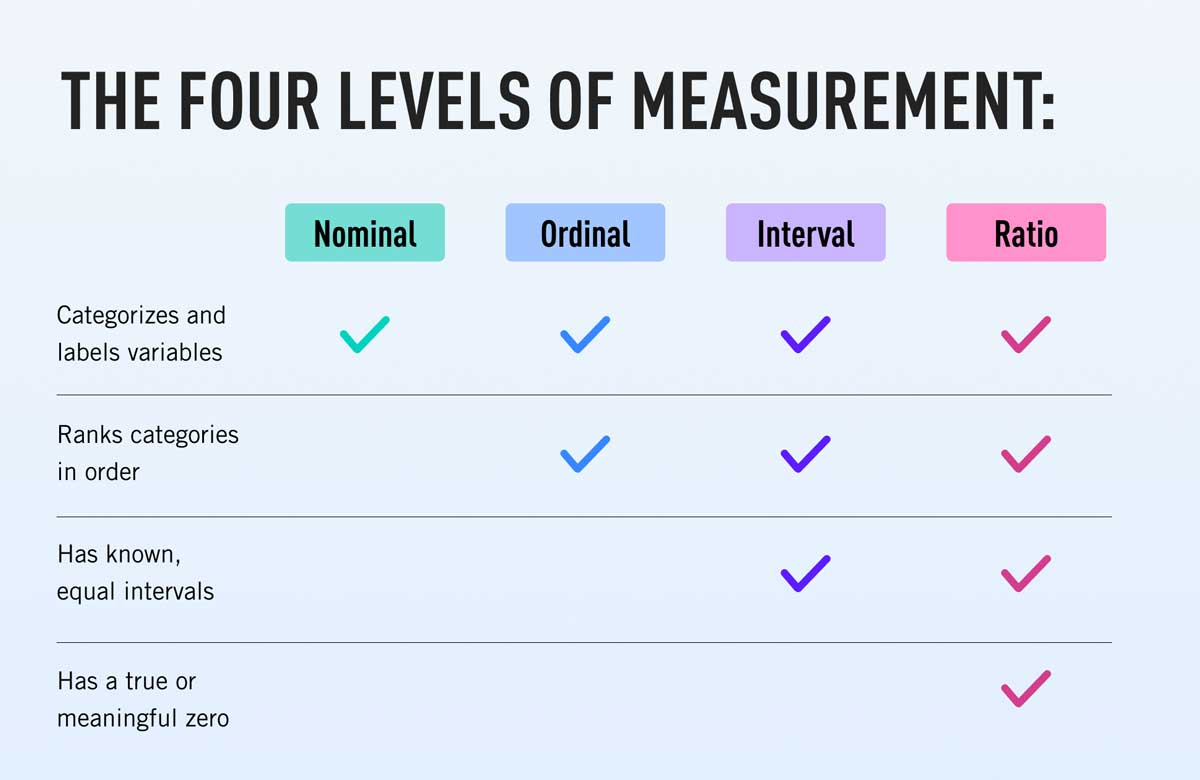
\includegraphics[width=0.7\textwidth]{Figure0102.jpg}
        \caption{Level of measurements.}
        \label{lec_01_fig02}
\end{figure}

\begin{ex-box}
    \noindent \pmb{Temperature Measurements as Interval and Ratio Values}.
    
    Temperature is an interesting physical quantity for understanding `interval' or `ratio' data. It turns out that it depends on the 'unit' you choose, or more intrinsically, the physical `scale' or `gauge' you choose.

    If measured in Fahrenheit or Celsius, the degree can range from negative to positive values, including zero. In this case, if two temperature measurements are taken, say today is 40 degrees (Fahrenheit) and yesterday was 20 degrees (Fahrenheit), one cannot say that today is twice as hot as yesterday. It is easy to see that if it is in terms of Celsius, the two numbers are 4.4 degrees and -6.8 degrees. The ratio becomes negative! In addition, with the two scales, 'zero' is meaningless; it can be anywhere if yet another modified temperature system is created.

   However, if scaled in terms of Kelvin, the absolute zero degree is physically defined \footnote{Kelvin zero is the lowest limit of the thermodynamic temperature scale, a state at which the entropy of a cooled ideal gas reaches its minimum value.}. Under this physical origin, two temperatures in Kelvin can be compared using a ratio (e.g., a 40K temperature is twice as hot as a 20K temperature).

\end{ex-box}

\subsection{Data vs Labels vs Features}
Given a data point, as seen previously $(\bm{x}_i,y_i)$, it may look ``machine-learning ready.'' However, in practice it is often not.

\textbf{Labels ($y_i$).} To obtain a categorical label $y_i$, we may label data with unranked (nominal) or ranked (ordinal) values. If the outcome is measured as a numerical quantity, it is common to convert it into categories via a rule (e.g., if $y_{i,\text{measured}} > 100$, then $y_i = \text{``Hot''}$).

\textbf{Features ($\bm{x}_i$).} Raw numerical measurements are not always good ``features'' directly. Data cleaning and feature preprocessing (scaling/transformations) are often needed so that different variables have comparable magnitudes and so that learning algorithms behave well.

\begin{itemize}
    \item \textbf{Interval $\leftrightarrow$ ratio transforms.} For positive ratio data $x>0$, a logarithm turns it into an interval-like variable: $y=\log(x)$. Conversely, an exponential can map interval values back to positive ratio values: $x=\exp(y)$.

    \item \textbf{Standardization (z-score scaling).} Given a feature $x$ with sample mean $\mu$ and standard deviation $\sigma$,
    \[
    z = \frac{x-\mu}{\sigma}.
    \]
    After standardization, the feature has approximately zero mean and unit variance.

    \item \textbf{Normalization (rescaling).} A common choice is min--max normalization to $[0,1]$:
    \[
    x' = \frac{x-x_{\min}}{x_{\max}-x_{\min}}.
    \]
    Another common choice is \textit{unit-norm} normalization for a vector-valued input $\bm{x}_i$:
    \[
    \bm{x}_i' = \frac{\bm{x}_i}{\lVert \bm{x}_i \rVert_2}.
    \]
\end{itemize}

\section{Notations and Dimensionality}
Nowadays, most sensors are digital, yet analog ones are still used. The differences are simple: digital data output discrete (numeric) data, while analog sensors produce continuous (numeric) data, as discussed above. In practice, continuous data is always digitized, leading to discrete data for digital processing and understanding. 

Besides representing and storing data using notations, an essential notion is \textit{dimensionality}. To understand these concepts and their intricacy, let's conduct a `thought experiment': monitoring the concrete strength of a critical infrastructure (e.g., a hydraulic dam).

\begin{ex-box}
    \noindent \pmb{Monitoring concrete strength for a hydraulic dam}. 
    
    This imagined experiment assumes that the inspector has access to sufficient resources to measure concrete strength. By standard codes, concrete strengths are measured at the $28^{th}$ day, at which the design strength should reach. In this experiment, the concrete is designed to have a nominal strength of $f'_c = 4 ksi$. Due to the critical importance of the structure (as a river-crossing dam with critical power generation and flood control functions), its strength will be continuously monitored in its lifecycle.
    
    The following schemes of different levels of complexity are designed:
\begin{enumerate}
\item [1)] A single measurement at the $28^{th}$ day at a single location. In this case, one measurement is obtained. 

\item [2)] 10 measurements at the $28^{th}$ day at the same single location. In this case, 10 measurements are obtained. 

\item [3)] A single measurement at a single location but measured at the $28^{th}$ day, then measured every month for two years. In this case, a single measurement at each date is obtained, and a total of 25 measurements is obtained.

\item [4)] A single measurement at a grid of locations ($10 \times 10$ or 100 locations) and measured at the $28^{th}$ day only. In this case, a single measurement is obtained at each location, for a total of 100 measurements.

\item [5)] A single measurement at a grid of locations ($10 \times 10$ or 100 locations) and measured at the $28^{th}$ day and every month after that for two years. In this case, a single measurement is obtained at each location and each date, for a total of 100 measurements at each date and $100 \times 25$ measurements overall.
\end{enumerate}

How do we describe the data above using mathematical symbols? Corresponding to the experiment schemes above, we tabulate how to represent them below (starting from Scheme S1 to S6).
\end{ex-box}



% Please add the following required packages to your document preamble:



\begin{table}[ht]
\begin{tabular}{|l|p{2in}|l|l|p{2in}|} % p{3in} does not work with multi-row environment
\hline
Scheme & Notation (using set and fake values)                                                                                                                & DP dim. & Data set size             & Graphical Illustration                                                                                                                                                                      \\ \hline
S1     & $\bm{f}=\{4.2\}$                                                                                                    & 1       & 1                         & A single 1D data point in an 1-D concrete-strength axis                                                                                                                                     \\ \hline
S2     & $\bm{f} =\{4.2, 4.1,... 3.9\}$                                                                                      & 1       & $1\times 10$                        & 10 single 1D data points in an 1-D concrete-strength axis                                                                                                                                   \\ \hline
S3     & $\bm{f} =\{4.2, 4.1,... 3.9\}$, $\bm{t} =\{1, 2,... 25\}$                                                       & 1       & $1 \times 25$             & 10 single 1D data points with 10 time-stamps, leading to a time series plotted in a 2-D Euclidean space                                                                                     \\ \hline
S4     & $\bm{F} =\{(4.2, 4.1,... 3.9); ...$, $(4.3,3.0, ... 4.1)\}$                                                           & 1       & $ 10 \times 10$           & 100 1D data points in a 2-D grid of $10\times 10$ locations, leading to a matrix (or an image). If plotted, leading to a surface plot in a 3-D Euclidean space                              \\ \hline
S5     & $\bm{F} =\big\{ \{(4.2, 4.1,... 3.9); ...$, $; (4.3,3.0, ... 4.1)\}$; $\{...\}$, $\{(4.0, 4.3,... 4.4); ...$, $; (3.3,4.0, ... 3.9) \big\}$, $\bm{t} =\{1, 2,... 25\}$ & 1       & $ 10 \times 10 \times 25$ & 2500 1D data points in a 2-D grid of $10\times 10$ locations and at 25 different time stamps, leading to 25 matrices. If plotted, leading to stacked surface plots in a 4-D Euclidean space \\ \hline
\end{tabular}
\caption{Data measurements and notations from a concrete-strength monitoring `thought' experiment. }
\label{Tab01}
\end{table}


Several comments are given below based on Table~\ref{Tab01}.

\begin{ex-box}
\noindent \pmb{Measurement vs sample dimension vs data set size}.

In ML, it is helpful to distinguish three related (but different) notions:
\begin{itemize}
\item \textbf{Measurement is scalar.} In this thought experiment, at a fixed time and location, the concrete strength measurement is a single number (a scalar).
\item \textbf{Sample/feature dimension $d$.} A single ML input $\bm{x}_i \in \mathbb{R}^d$ may collect many scalar measurements into one vector. For example, a $10\times 10$ spatial grid of scalar measurements can be represented as a matrix, or equivalently flattened into a vector with $d=100$ features.
\item \textbf{Data set size $n$.} The number of samples in a data set (e.g., the number of time stamps, locations, or experiments) is typically denoted by $n$.
\end{itemize}

Therefore, even if each \emph{individual measurement} is scalar, a single \emph{ML sample} $\bm{x}_i$ can be high-dimensional when we aggregate many measurements into one input.
\end{ex-box}

\begin{itemize}
\item All data points are 1-D - at a time and at a location, and a scalar-valued measurement is obtained.
\item Under S2 and S3, vector notations can be used to describe the set. In this case, we can use a row vector. In linear algebra, the dimension of a vector is its size, which can be treated as a 'data point' in Euclidean space or a vector in a vector space. However, our physical data point here, the measurement at each location and each time, is still 1-D. Multi-dimensional data points from physical measurements are discussed later.

Also noted in S3, given the time stamps as a set or a vector of the same size, we achieve a time series. One can plot the time-series in a 2-D space, one axis is the time ($t$), and the other is the concrete strength ($f'_c$).

\item It is noted that in the cases of S4 and S5 above, a matrix of measurements is obtained at a time. A 2D matrix array notation can be used for the data set, which is
\begin{equation*}
\bm{F} = 
\begin{bmatrix}
4.2 & 4.1 & ... & 3.9\\
... & ... & ... & ...\\
4.3 & 3.0 & ... & 4.1
\end{bmatrix}
\end{equation*}
which is a $10\times 10$ matrix.

In S4, data points in a 2D matrix can be visualized as a surface plot. Note that in this case, the axes are the $x$ and $y$, and the third axis is $f'_c$.

\item Under S5, the set notation tells that there is a time series of measurement matrices, leading to $10\times 10 \times 25$ data points. A nested matrix notation can be used:

\begin{equation*}
\bm{F} = \left\{
\begin{bmatrix}
4.2 & 4.1 & ... & 3.9\\
... & ... & ... & ...\\
4.3 & 3.0 & ... & 4.1
\end{bmatrix}
,...,
\begin{bmatrix}
4.0 & 4.3 & ... & 4.4\\
... & ... & ... & ...\\
3.3 & 4.0 & ... & 3.9
\end{bmatrix}
\right\}
\end{equation*}
which nests a total of 25 $10\times 10$ matrices when considering the 25 dates.

To plot this, bedsides the 3-D coordinate system $x - y - f'_c$, a time axis $t$ is further needed. This can be done by shifting one $x - y - f'_c$ at a time to another time, when a time axis is added. To this end, we see that data visualization becomes challenging.
\end{itemize}


A data point can be physically high-dimensional, i.e., a vector. Still using the thought experiment above, we now introduce another scheme.

\begin{ex-box}
\noindent \pmb{Vector data points}

In this scheme, the inspector uses three techniques to measure concrete strength at each location and each time (e.g., Drilled Core, a destructive test; two non-destructive tests: Rebound Hammer and Penetration Resistance Test). To simplify it, the inspector conducts these tests only at a linear 10 locations, it will lead to an array in this form (using some fake data):
\[
\bm{f} = \{ (4.1, 3.9, 4.0)^T, (2.0, 2.8, 3.0)^T, ..., (4.1, 5.0, 4.2)^T \}\
\]
where a data point is 3-dimensional. In a matrix form, it is 

\begin{equation*}
\bm{F} = 
\begin{bmatrix}
4.1 & 2.0 & ... & 4.1\\
3.9 & 2.8 & ... & 5.0\\
4.0 & 3.0 & ... & 4.2
\end{bmatrix}
\end{equation*}
where each data point is expressed as a $3\times 1$ column vector. Although similar to the one used for S4, this matrix notation bears a different physical meaning. The column vector is treated as a data point. 

If it goes further, for example, the monitoring continues at different times. There is no better way to express the data, and one way looks like this:
\begin{equation*}
\bm{F} = 
\left\{\begin{bmatrix}
4.1 & 2.0 & ... & 4.1\\
3.9 & 2.8 & ... & 5.0\\
4.0 & 3.0 & ... & 4.2
\end{bmatrix},
...,
\begin{bmatrix}
4.0 & 4.0 & ... & 4.1\\
3.7 & 3.8 & ... & 4.0\\
2.8 & 5.0 & ... & 3.2
\end{bmatrix} \right\}
\end{equation*}
Again, though it is similar to the nested matrix for S5, the physical meaning is different.
\end{ex-box}

Lastly, to simplify the notation, we consider a linear set of locations for the vector-valued measurements above. If a matrix of locations is used, the nesting will be vertical. In modern ML practices, the concept of \textit{tensor} is often used to handle high-dimensional, complex data. We will return to this when introducing deep learning (DL) frameworks.



\section{Special Data: Imagery Data}

We conclude this topic by introducing a special data type: imagery data. Images or imagery data are collected in many instances. Going back to the concrete monitoring project above, a meaningful activity in civil structures management practice besides' strength' monitoring is damage assessment. Visual assessment (by engineers' naked eyes) still dominates practice. Nonetheless, machine vision, or computer vision (ML applied to imagery data), has been extensively researched. Inspection automation with robotic platforms is on the horizon. Other examples in common machine vision practice include facial recognition, character recognition, and natural-scene understanding. Another significant example is remote sensing, where aerial or satellite sensors provide large-scale imagery of the Earth. 

\begin{ex-box}
\noindent \pmb{Practical tensor shapes for images and videos}.

In modern ML/DL libraries, imagery data is stored as tensors (multi-dimensional arrays). Common conventions include:
\begin{itemize}
\item Grayscale image: shape $(H,W)$.
\item Color image: shape $(H,W,C)$, where $C=3$ for RGB.
\item Video: shape $(T,H,W,C)$, where $T$ is the number of frames.
\item Mini-batch of data: often adds a leading batch dimension $N$, e.g., $(N,H,W,C)$ for images and $(N,T,H,W,C)$ for videos.
\end{itemize}

Note: in ML, the word \textit{rank/order} of a tensor refers to the number of axes (dimensions) above, which is different from the \textit{matrix rank} in linear algebra. We return to tensor concepts and notation in \textbf{Appendix B}.
\end{ex-box}

In the following, we use a sample satellite image to illustrate its storage structure for three common image types: binary (black-and-white), gray (intensity), and color (red, green, and blue bands). An image is often digitally stored using matrices. A pixel is a digital `data point' that is measured at a location in an imaging plane (which physically means the CCD chip in a digital camera). An image is described by its size, for example, $100 \times 200$, meaning that it has 100 rows and 200 columns, hence $100 \times 200$ pixels. 

\begin{figure}
     \centering
     \begin{subfigure}[b]{0.4\textwidth}
         \centering
         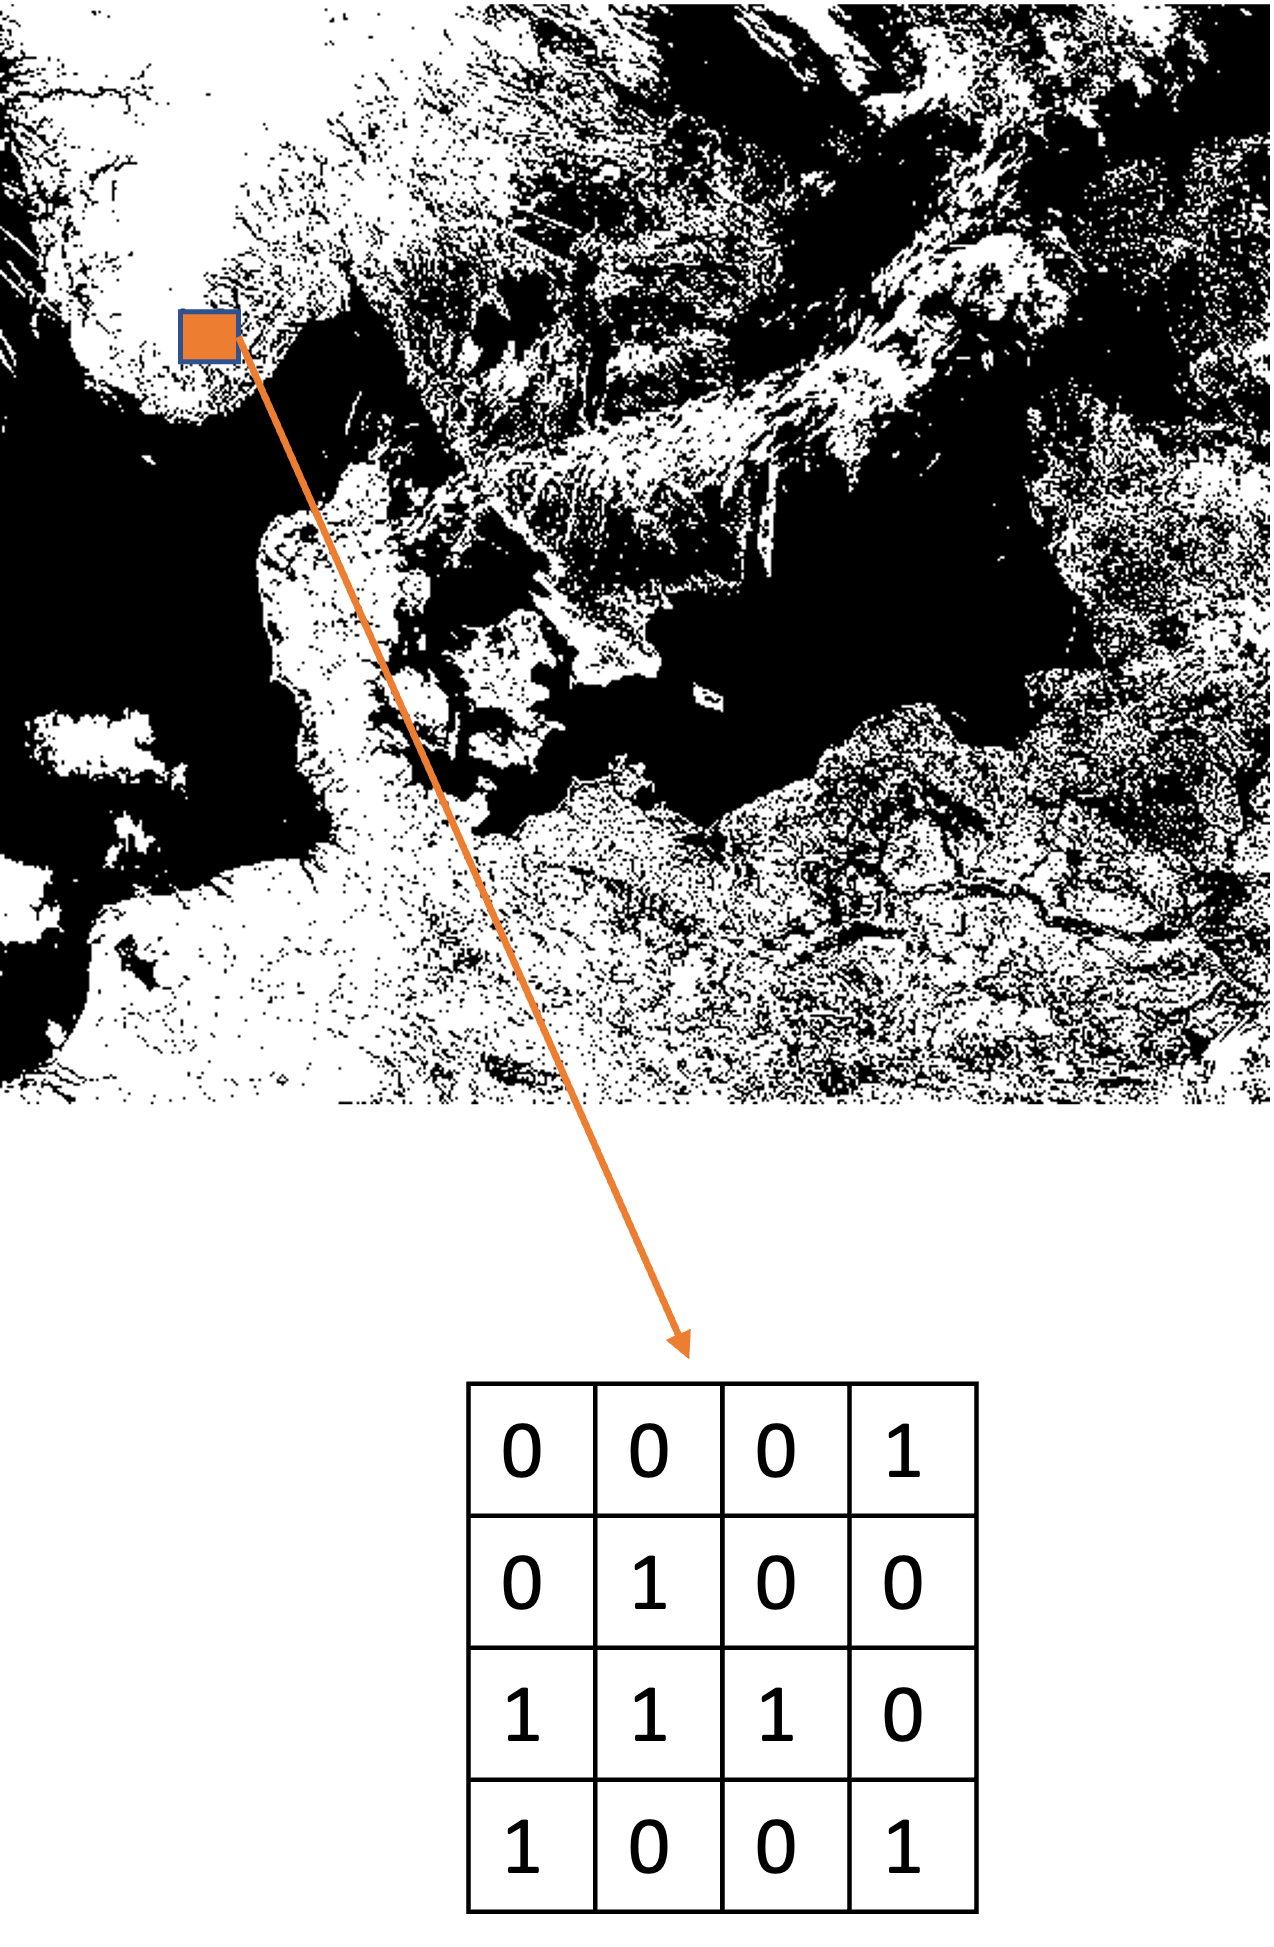
\includegraphics[width=\textwidth]{Figure0104a.png}
         \label{lec_01_fig04a}
         \caption{}
     \end{subfigure}
     \hfill
    \begin{subfigure}[b]{0.4\textwidth}
         \centering
         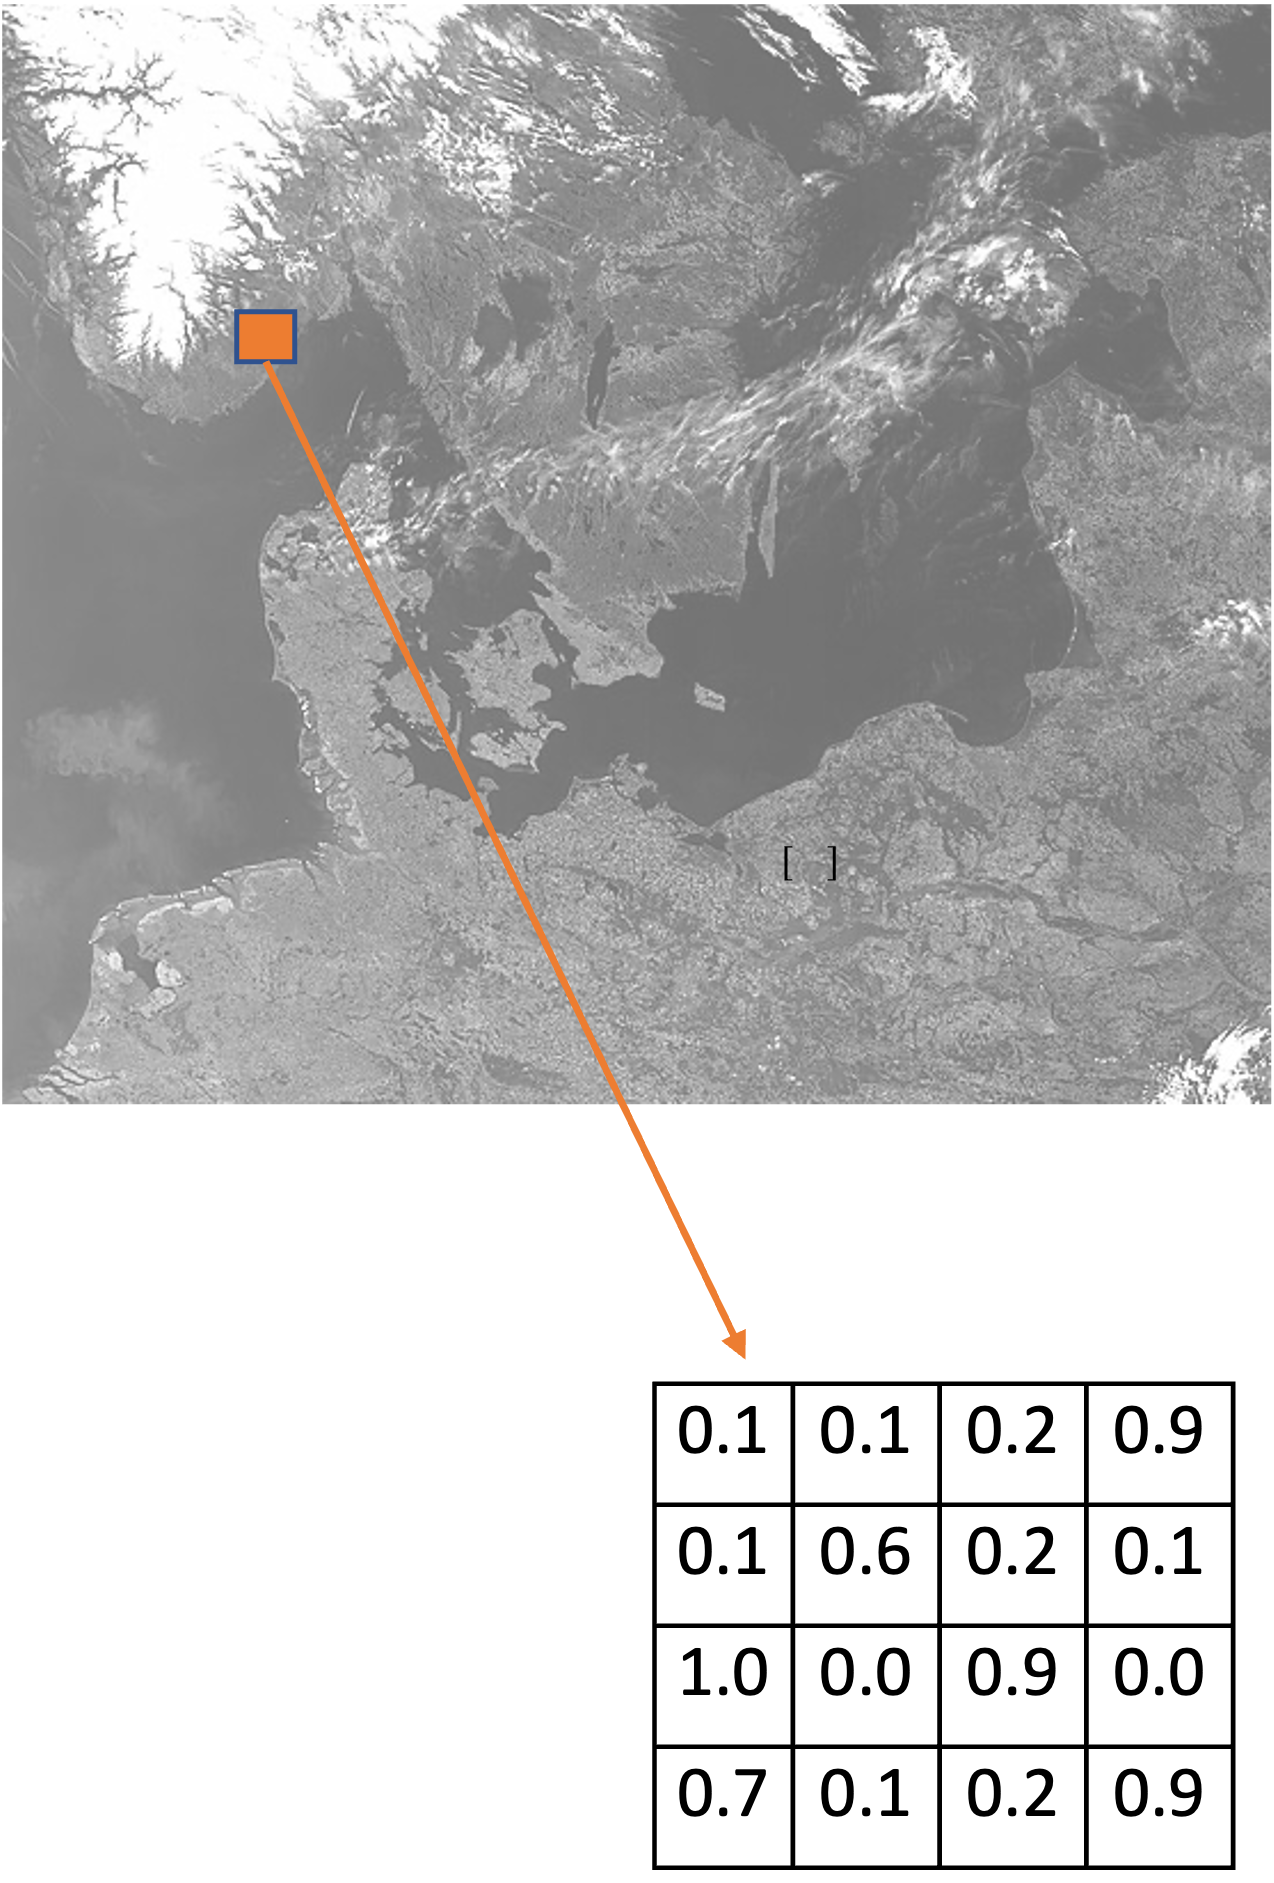
\includegraphics[width=\textwidth]{Figure0104b.png}
         \label{lec_01_fig04b}
         \caption{}
     \end{subfigure}
     \hfill
       \begin{subfigure}[b]{0.5\textwidth}
         \centering
         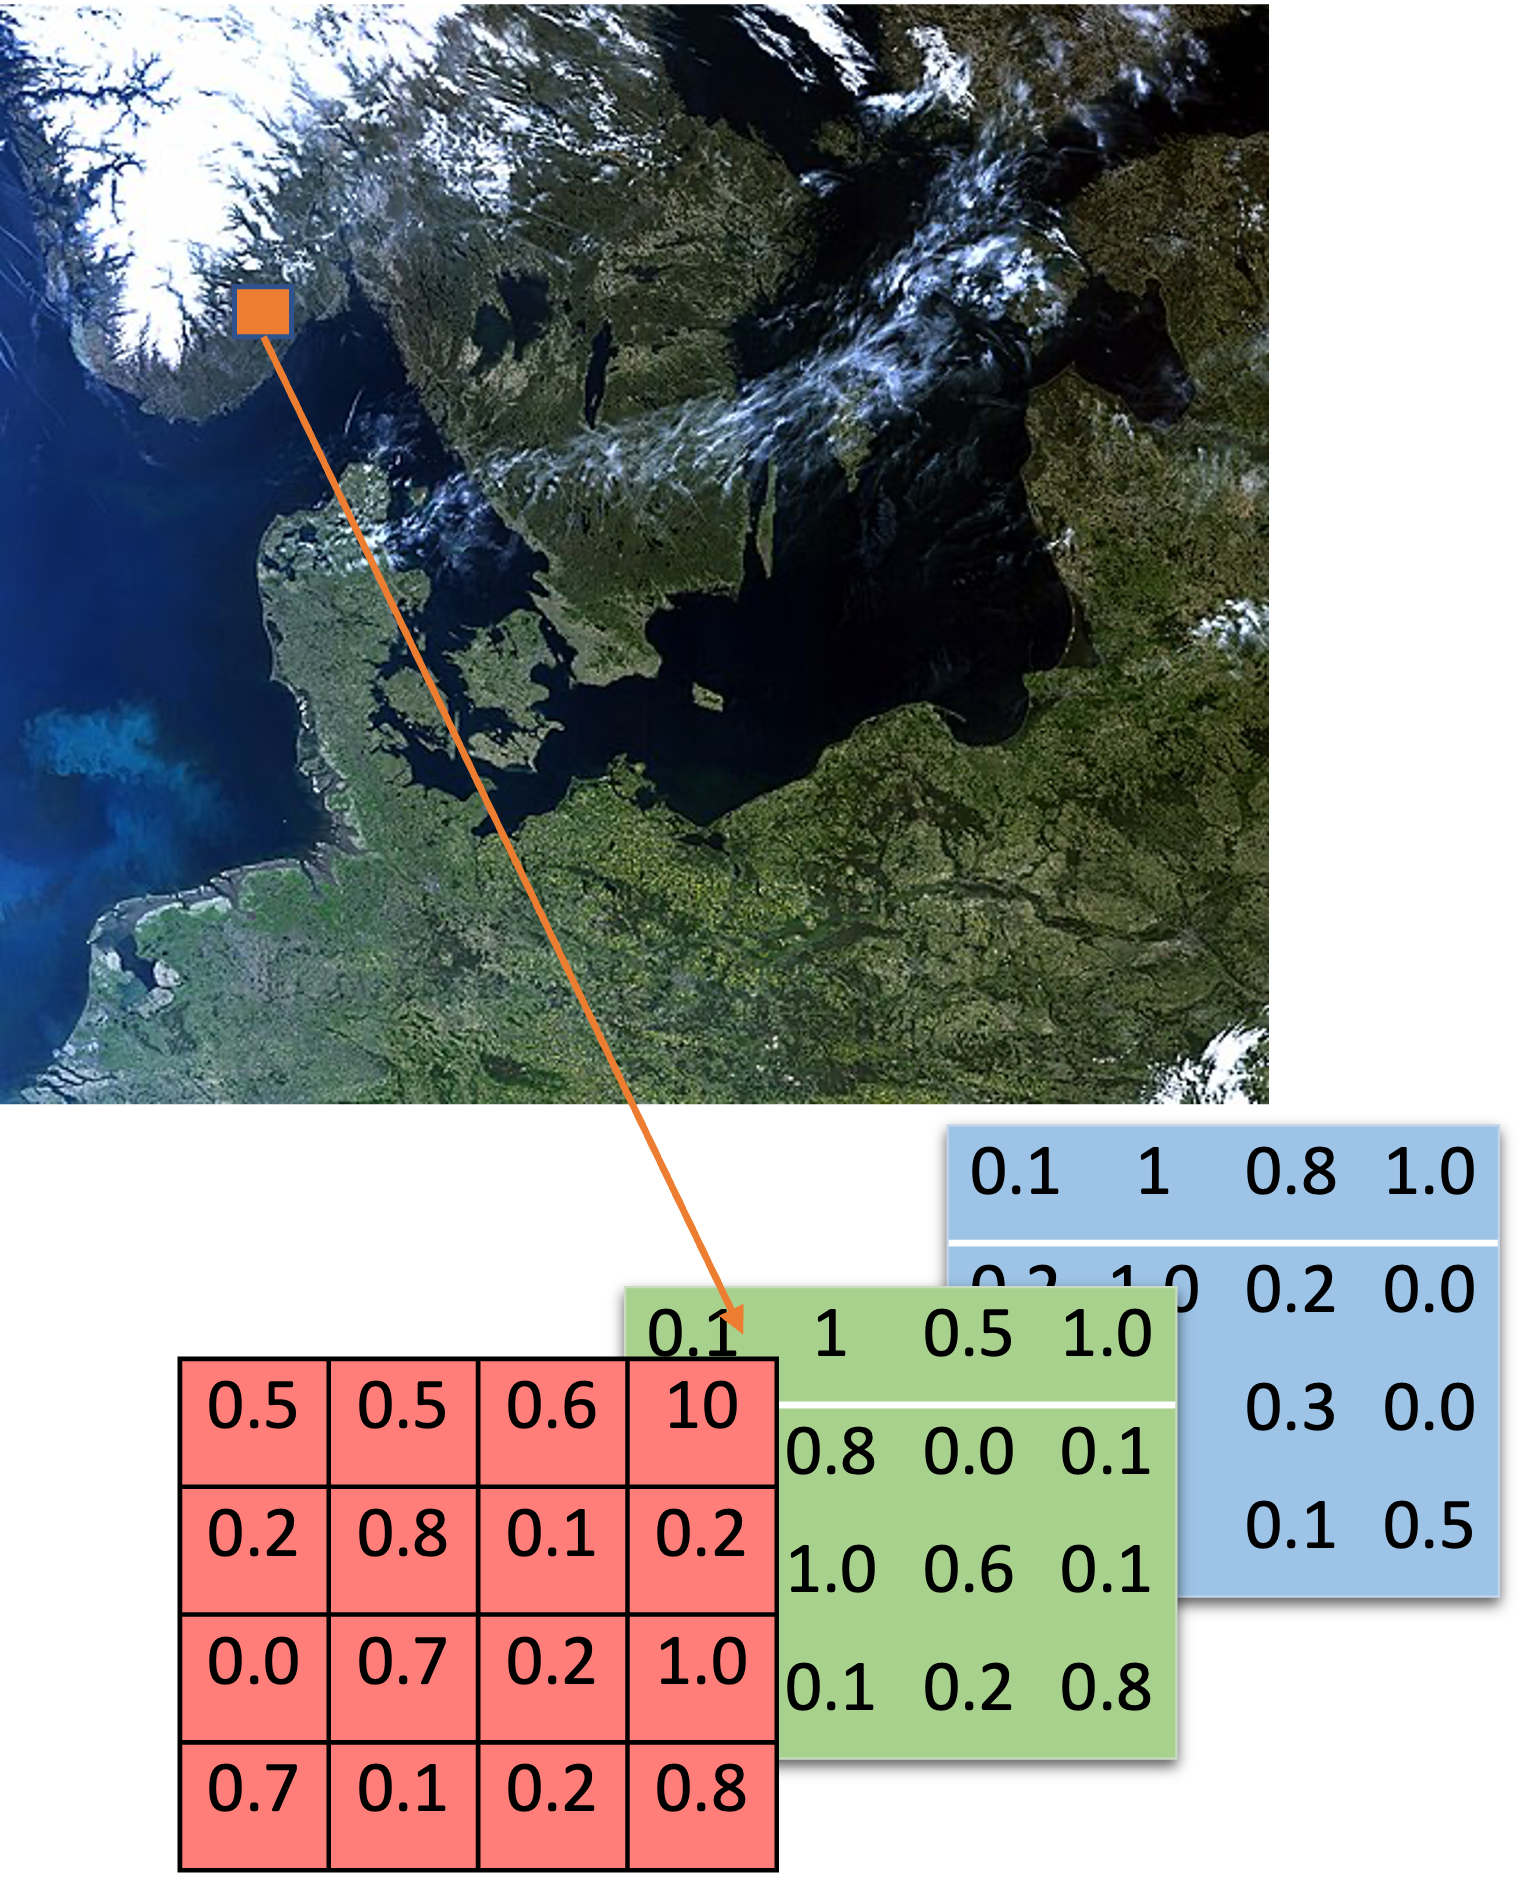
\includegraphics[width=\textwidth]{Figure0104c.png}
         \label{lec_01_fig04c}
         \caption{}
     \end{subfigure}

\caption{Illustration of images and matrix structures: (a) binary image; (b) gray image; (c) color image}
\label{lec_01_fig04}
\end{figure}

The original images shown in Fig.~\ref{lec_01_fig04} have a size of $550 \times 480$ (550 rows and 480 columns) in terms of matrices. Their values and types are different at each pixel. 

\begin{enumerate}
\item [a.] In a binary (black-and-white) image, a matrix element, or pixel, is binary-valued, taking 0 (black) or 1 (white). A small image patch ($4 \times 4$) is illustrated here.
\item [b.] In the gray image, a matrix element or a pixel has a numeric value. In this case, it changes from 0 to 1, producing a range of gray levels from black to white. In imaging science, integer values can be used. For example, to represent 256 gray levels, 0-255 are used. A small image patch ($4 \times 4$) is also illustrated in this way.

\item [c.] The color image is shown later. A color image is produced when the imaging sensor collects intensity values across three primary color bands: red, green, and blue. Therefore, a three-layer matrix is obtained. Using $0 ~ 1$ as the intensity values at the three bands,  a small image patch ($4 \times 4$) taken from the image is illustrated too, and three matrices are expressed in the order of red, green, and blue.
\end{enumerate}

We can see the similarity between the image and the concrete strength monitoring experiment above (which collects measurements at an array of locations in the $x$ and $y$ directions). When we collect three different values at a location using three different instruments, the resulting measurements can be imagined as analogous to a `color' image.

We leave a question here. How to express using matrix notations about video data? The hint is that video means a time series of image frames. 




\newpage
\appendix
\section*{Appendix A: Basic Linear Algebra Notations and Concepts}

\subsection*{Vectors and Matrices}
\begin{itemize}
    \item A \textbf{vector} in $\mathbb{R}^n$ is often written as 
    \[
        \bm{v} = 
        \begin{pmatrix}
            v_1 \\ 
            v_2 \\ 
            \vdots \\ 
            v_n
        \end{pmatrix}.
    \]
    \item A \textbf{matrix} $\bm{A}$ of size $m \times n$ can be written as:
    \[
        \bm{A} = 
        \begin{pmatrix}
            a_{11} & a_{12} & \dots & a_{1n} \\
            a_{21} & a_{22} & \dots & a_{2n} \\
            \vdots & \vdots & \ddots & \vdots \\
            a_{m1} & a_{m2} & \dots & a_{mn}
        \end{pmatrix}.
    \]
\end{itemize}

\subsection*{Special Matrices}
\begin{itemize}
    \item A matrix $\bm{A}$ is \textbf{symmetric} if $\bm{A} = \bm{A}^\top$, i.e., $a_{ij} = a_{ji}$ for all $i, j$.
    \item The \textbf{identity matrix} of size $n \times n$, denoted $I_n$, is given by
    \[
        \bm{I} = 
        \begin{pmatrix}
            1 & 0 & \dots & 0 \\
            0 & 1 & \dots & 0 \\
            \vdots & \vdots & \ddots & \vdots \\
            0 & 0 & \dots & 1
        \end{pmatrix}.
    \]
    \item A matrix is called \textbf{sparse} if most of its entries are zero. For example,
    \[
        \bm{S} = 
        \begin{pmatrix}
            0 & 0 & 1 \\
            0 & 0 & 0 \\
            2 & 0 & 0
        \end{pmatrix}
    \]
    is sparse because it contains many zeros.
\end{itemize}

\subsection*{Rank, Determinant, and Inverse of Square Matrices}
\begin{itemize}
    \item The \textbf{rank} of a matrix $\bm{A}$, denoted $\mathrm{rank}(A)$, is the dimension of its column space (or row space). 
    \item The \textbf{determinant} of a square matrix $\bm{A}$ (of size $n \times n$) is denoted $\det(\bm{A})$ or $|\bm{A}|$. 
        \[
            \det(\bm{A}) \neq 0 \quad \Longleftrightarrow \quad \text{the matrix $\bm{A}$ is invertible (non-singular).}
        \]
    \item The \textbf{inverse} of a non-singular matrix $\bm{A}$ is the unique matrix $A^{-1}$ such that
        \[
            \bm{A} \bm{A}^{-1} = \bm{A}^{-1} \bm{A} = \bm{I}.
        \]
\end{itemize}

\subsection*{Solving Linear Systems}
\begin{itemize}
    \item A \textbf{linear system} in matrix form is written as:
    \[
        \bm{A} \bm{x} = \bm{b},
    \]
    where $\bm{A}$ is an $n \times n$ matrix, $\bm{x}$ is the unknown vector in $\mathbb{R}^n$, and $\bm{b}$ is a known vector in $\mathbb{R}^n$.
    \item \textbf{Conditions for unique solutions:}
    \[
        \det(\bm{A}) \neq 0 \quad \Longleftrightarrow \quad A \text{ is non-singular} 
        \quad \Longleftrightarrow \quad \mathrm{rank}(A) = n \quad \Longleftrightarrow \quad \text{system has a unique solution}.
    \]
    \item If $\det(\bm{A}) = 0$, $\bm{A}$ is \textbf{singular}, and the system may have either no solutions or infinitely many solutions, depending on $\mathrm{rank}(A)$ and the augmented system.
\end{itemize}

\subsection*{Rectangular Matrices and the Pseudo-Inverse}

Consider $A$ as an $m \times n$ matrix:
\begin{itemize}
    \item \textbf{Pseudo left inverse}: If $m \ge n$ and $A$ has \emph{full column rank} ($\mathrm{rank}(A) = n$), then 
    \[
        A_\ell^+ = (A^\top A)^{-1} A^\top
    \]
    is a left inverse of $A$, since 
    \[
        A_\ell^+ A = I_n.
    \]
    \item \textbf{Pseudo right inverse}: If $m \le n$ and $A$ has \emph{full row rank} ($\mathrm{rank}(A) = m$), then 
    \[
        A_r^+ = A^\top (A A^\top)^{-1}
    \]
    is a right inverse of $A$, because 
    \[
        A\, A_r^+ = I_m.
    \]
\end{itemize}
In both cases, these matrices serve as specialized inverses that apply when $A$ is rectangular rather than square. 

\subsection*{Linear Regression and Least-Squares Solutions}
\begin{itemize}
    \item In linear regression, one often solves
    \[
        X \boldsymbol{\beta} = \mathbf{y},
    \]
    where $X$ is an $m \times n$ matrix of predictors (with $m$ data points and $n$ predictors), $\boldsymbol{\beta}$ is an $n \times 1$ vector of unknown coefficients, and $\mathbf{y}$ is an $m \times 1$ vector of observed responses.
    \item When $m \ge n$ and $X$ has full column rank (i.e., $\mathrm{rank}(X)=n$), the \textbf{ordinary least-squares} (OLS) solution for $\boldsymbol{\beta}$ is given by:
    \[
        \boldsymbol{\beta} = (X^\top X)^{-1} X^\top \mathbf{y}.
    \]
    Notice that $(X^\top X)^{-1} X^\top$ is precisely a \emph{pseudo left inverse} of $X$ in this scenario.
    \item If $m \le n$ and $X$ has full row rank (i.e., $\mathrm{rank}(X)=m$), one can use the \textbf{pseudo right inverse} $X^\top (X X^\top)^{-1}$ to seek a least-squares solution (particularly in cases of an ``underdetermined'' system). 
    \item More generally, if $X$ is not necessarily full column or full row rank, we can use the \textbf{Moore-Penrose pseudo-inverse} $X^+$ to find a least-squares solution:
    \[
        \boldsymbol{\beta} = X^+ \mathbf{y}.
    \]
    The Moore-Penrose pseudo-inverse unifies these cases and ensures a (minimum-norm) least-squares solution.
\end{itemize}

\newpage
% ====================== Tensor Section ======================
\section*{Appendix B: Tensors in Machine Learning}

Modern machine learning (ML) and deep learning (DL) frameworks like \textbf{TensorFlow}, \textbf{PyTorch}, and \textbf{JAX} rely on tensors as their core data structure. Tensors generalize scalars, vectors, and matrices to arbitrary dimensions, enabling efficient representation of complex data (e.g., images, videos, time-series) and model parameters (e.g., neural network weights).

\subsection*{Definition}
A \textbf{tensor} is a multi-dimensional array of numerical values. Formally:
\begin{itemize}
    \item \textbf{Rank/Order}: Number of dimensions (e.g., rank 0 = scalar, rank 1 = vector).
    \item \textbf{Transformation Rules}: In physics/math, tensors obey coordinate-invariant laws. In ML/DL, they primarily serve as $n$-dimensional data containers.
\end{itemize}

\subsection*{Notation}
\begin{itemize}
    \item \textbf{Symbols}: Boldface for tensors (e.g., $\bm{T}$ for matrices, $\mathcal{T}$ for rank $\geq 3$).
    \item \textbf{Components}: $T_{ijk\dots}$ denotes a specific element in the tensor.
    \item \textbf{Einstein Summation}: Implicit summation over repeated indices:
    \[
    C_{ik} = A_{ij} B_{jk} \equiv \sum_j A_{ij} B_{jk}
    \]
\end{itemize}

\subsection*{Examples by Rank}
\begin{itemize}
    \item \textbf{Rank 0 (Scalar)}: $T = 5.2$ 
    \item \textbf{Rank 1 (Vector)}: $\bm{v} = [v_1, v_2, \dots, v_n]$
    \item \textbf{Rank 2 (Matrix)}: Neural network weights $\bm{W} = [W_{ij}]$
    \item \textbf{Rank 3}: RGB image $\bm{I}_{ijk}$ (height $\times$ width $\times$ channels)
    \item \textbf{Rank 4}: Video batch $\mathcal{B}_{ijkl}$ (batch size $\times$ height $\times$ width $\times$ frames)
\end{itemize}

\subsection*{Tensor Representations of Sensor Data}
\begin{table}[ht]
\centering
\caption{Sensor data types as tensors}
\label{tab:sensor_data}
\begin{tabular}{|l|l|l|}
\hline
\textbf{Dimension} & \textbf{Structure} & \textbf{Examples} \\ \hline
1D & $\{ u_i \mid i = 1, 2, \dots, I \}$ & Temperature readings, stock prices \\ \hline
2D & $\{ u(x_i, y_j) \}$ & Grayscale images, grid measurements \\ \hline
3D & $\{ u(x_i, y_j, t_k) \}$ & Video (2D + time), MRI scans \\ \hline
4D & $\{ u(x_i, y_j, s_k, t_l) \}$ & Hyperspectral video (3D + time) \\ \hline
\end{tabular}
\end{table}

\subsection*{Key ML/DL Applications}
\begin{itemize}
    \item \textbf{Neural Networks}: Weights/biases stored as tensors.
    \item \textbf{GPU Acceleration}: Frameworks like TensorFlow use tensors for parallel computation.
    \item \textbf{Autograd}: Automatic differentiation (e.g., $\nabla_{\bm{W}} \mathcal{L}$ for gradient descent).
\end{itemize}


\end{document}
